\section*{Oppgave 1: Denoise i Python og Numpy+Weave}

Python-implementasjonen er basert på algoritmen som fantes i denoise.c. Algoritmen gjør som den skal, men er (som forventet) ganske treg.

Numpy-weave-implementasjonen derimot er ganske mye raskere. Jeg har delt opp implementasjonen av C-koden i to biter og lagt disse ut i en separat python-fil for å gjøre \verb;numpy_weave.py; litt ryddigere. Koden finnes i src/denoise/weave\_c.py, og er delt i denoise\_c og support\_c, der den siste inneholder typedefs og funksjoner som brukes i denoising og manipulering.

I oppgaveteksten var det nevnt at man skulle bruke timeit for å sammenligne de ulike backendene. Det sto ikke eksplisitt hvor det skulle gjøres, men ettersom flere backends skjeldent kjøres samtidig og man derfor ikke enkelt vil kunne få en sammenligning ved å kjøre det gjennom frontend implementerte jeg en sammenligningstest i \verb;test_speed_test.py;. Testen sammenligner bare svart-hvit-denoising siden dette er den logikken som finnes i alle tre backendene.

\subsection*{Resultat fra kjøring}
%@exec python test_speed_test.py

Det eneste overraskende med resultatet er at min numpy-weave-implementasjon ser ut til å være raskere enn denoise\_c.

Det er egentlig ikke tilfelle, og skyldes at jeg i implementasjon av den rene C-backenden starter med å gjøre en import av bildet for å finne ut om det er et fargebilde (for å kunne gi feilmelding om at farger ikke støttes av den backenden).

\subsection*{Denoising-eksempler med ulike backends}

Nedenfor vises originalbildet, og videre vises dette bildet denoiset med en kappa på 0.1 og 10 iterasjoner med de ulike backendene; numpy-weave, pure-python og til slutt fra denoise.c.

\begin{figure}[!h]
\centering
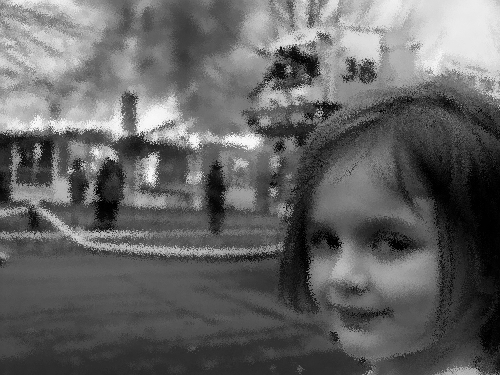
\includegraphics[width=90mm]{disasterbefore}
\caption{Original image \label{original}}
\end{figure}

\pagebreak

%@exec
python denoise.py disasterbefore.jpg out.jpg --kappa=0.1 --iter=10
%@

\begin{figure}[!h]
\centering
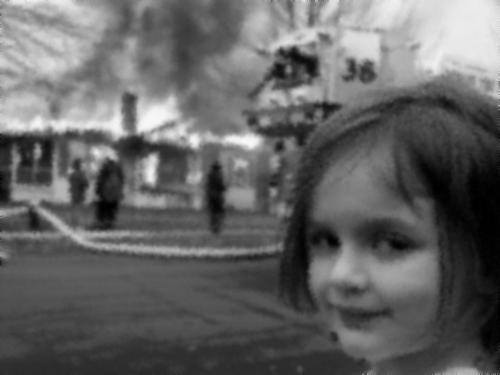
\includegraphics[width=90mm]{nw-01-10}
\caption{Denoised with numpy-weave, kappa=0.1, iter=10 \label{nw-mono}}
\end{figure}

\pagebreak

%@exec
python denoise.py disasterbefore.jpg out.jpg --kappa=0.1 --iter=10 --backend=python
%@

\begin{figure}[!h]
\centering
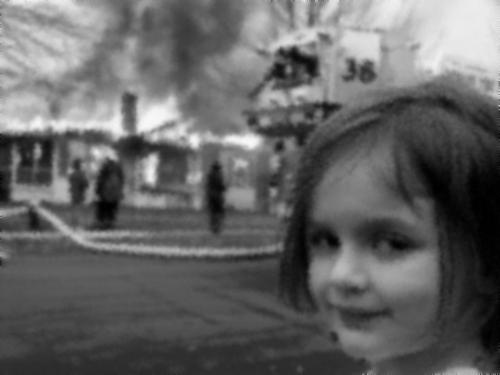
\includegraphics[width=90mm]{p-01-10}
\caption{Denoised with python, kappa=0.1, iter=10 \label{p-mono}}
\end{figure}

\pagebreak

%@exec
python denoise.py disasterbefore.jpg out.jpg --kappa=0.1 --iter=10 --backend=c
%@

\begin{figure}[!h]
\centering
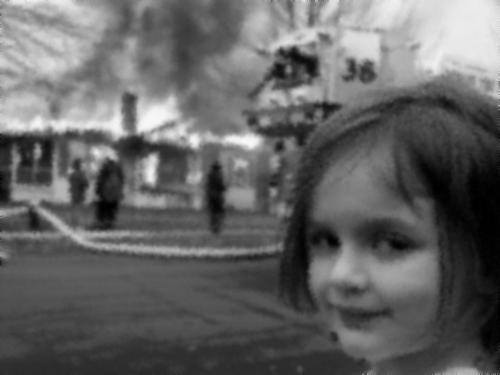
\includegraphics[width=90mm]{nw-01-10}
\caption{Denoised with denoise\_c, kappa=0.1, iter=10 \label{c-mono}}
\end{figure}

\pagebreak